\section{Theoretische Grundlagen}
\subsection{Biometrie}
TORBEN 
Bei der Biometrie handelt es sich um eine Wissenschaft, welche sich mit der Vermessung von menschlichen Merkmalen beschäftigt.
Die Ergebnisse dieser Messungen können dann dazu verwendet werden, Individuen zu beschreiben und zu identifizieren. Dieser Bereich 
der Biometrie wird auch als \textit{biometrische Erkennungsverfahren} beschrieben. Eine andere Facette der Biometrie, die \textit{biometrische Statistik},
beschäftigt sich mit der Auswertung der erfassten Daten um diese zur Analyse zu nutzen.
Mit der biometrischen Statistik, werden wir uns in dieser Studienarbeit beschäftigen, um die Merkmale, die mittels 
Smartphone erfasst werden, auszuwerten und damit Rückschlüsse auf die Emotionen eines Menschen zu ermöglichen.
\subsection{Smartphone}
sollte auch erklärt werden weil wir ja damit primär arbeiten
\subsection{Was sind Emotionen?}
TORBEN
Da wir uns in dieser Arbeit primär mit der Erkennung von Emotionen beschäftigen wollen, ist es wichtig den Begriff Emotion zu definieren.
Schwarzer-Petruck beschreibt in ihrem Werk Emotionen und pädagogische Professionalität eine Emotion als \textit{``ein komplexes
Muster körperlicher und mentaler Veränderungen als Antwort auf eine als persönlich bedeutsam wahrgenommene Situation''}\footcite[S.51 Z.20ff]{Sch13}.
Das Muster umfasst laut Schwarzer-Petruck die Aspekte des kognitiven Prozess, die Gefühle, eine Verhaltensreaktion und eine physiologische Erregung.
\subsection{Grundlagen der Emotionserkennung}
Ich schreibe etwas mal gucken bo was bassiert.
\subsection{Welche Möglichkeiten gibt es?}
\subsubsection{Nutzerinteraktionen}
Im Laufe des Alltags verwenden Nutzer ihr Smartphone sehr häufig. Dabei können unteranderem Aspekte wie das Tippverhalte, 
z. Bsp. verwendet der User viele Smileys, Rückschlüsse auf den emotionalen Zustand eines Nutzers ermöglichen.
\subsubsection{Im Smartphone eingebaute Sensoren}
\subsubsection{Zusätzliche Hardware}
Im Rahmen des Projektes wird die Möglichkeit erforscht, mit Hilfe eines Arduinos die Hautleitfähigkeit aufzuzeichnen. 
Diese ist ein großer Faktor bei der Bestimmung von Emotionen und wird unteranderem auch in Lügendetektoren verwendet. 
\begin{figure}[h]
	\centering
	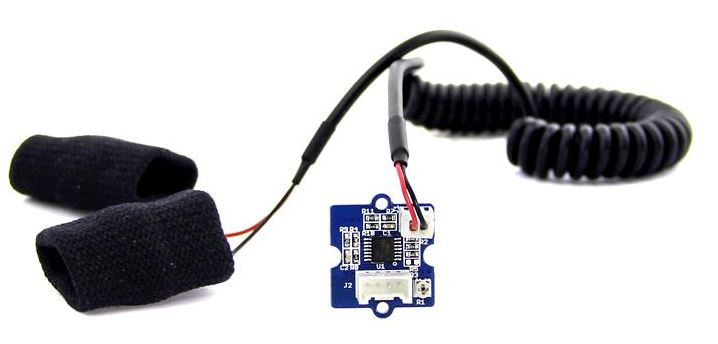
\includegraphics[width=11cm]{Bilder/sensor.jpg}
	\caption{Das ist ein cooler GSR Sensor}
\end{figure}%